\documentclass{beamer}

\usepackage{framed}
\usepackage{graphicx}

\begin{document}
%====================================%
\begin{frame}[fragile]
	\frametitle{Seaborn Workshop}
	\large 
	
	\begin{itemize}
\item Some plots benefit from offsetting the spines away from the data, which can also be done when calling \texttt{despine()}. 
\item When the ticks don’t cover the whole range of the axis, the trim parameter will limit the range of the surviving spines.

	\end{itemize}
\end{frame}
%====================================%
\begin{frame}[fragile]
	\frametitle{Seaborn Workshop}
	\large
	\begin{verbatim}
	f, ax = plt.subplots()
sns.violinplot(data)
sns.despine(offset=10, trim=True);
\end{verbatim}
\begin{figure}
\centering
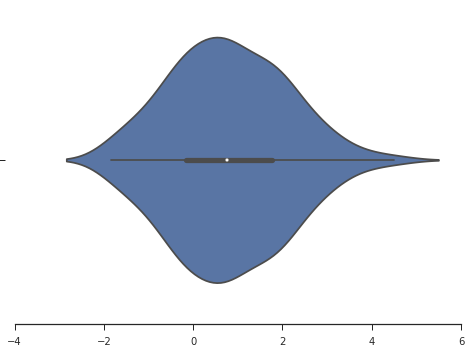
\includegraphics[width=0.7\linewidth]{images/aesthetics_23_0}
\end{figure}


\end{frame}
%====================================%
\begin{frame}[fragile]
	\frametitle{Seaborn Workshop}
	\large
You can also control which spines are removed with additional arguments to \texttt{despine()}:
\begin{verbatim}
sns.set_style("whitegrid")
sns.boxplot(data=data, palette="deep")
sns.despine(left=True)
\end{verbatim}

\begin{figure}
\centering
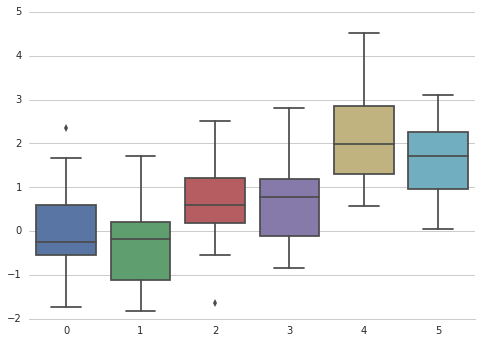
\includegraphics[width=0.6\linewidth]{images/aesthetics_25_0}
\caption{}
\label{fig:aesthetics_25_0}
\end{figure}


\end{frame}
\section{Temporarily setting figure style}
	%====================================%
\begin{frame}[fragile]
	\frametitle{Seaborn Workshop}
	\large
	\begin{itemize}
\item Although it’s easy to switch back and forth, you can also use the \texttt{axes\_style()} function in a with statement to temporarily set plot parameters. 
\item This also allows you to make figures with differently-styled axes:
	\end{itemize}

\end{frame}
%====================================%
\begin{frame}[fragile]
	\frametitle{Seaborn Workshop}
	\large
\begin{verbatim}
with sns.axes_style("darkgrid"):
plt.subplot(211)
sinplot()
plt.subplot(212)
sinplot(-1)
\end{verbatim}
\begin{figure}
\centering
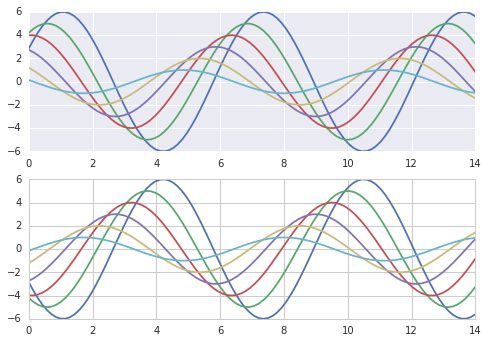
\includegraphics[width=0.7\linewidth]{images/aesthetics_27_0}
\end{figure}

\end{frame}
\section{Overriding elements of the seaborn styles}
%====================================%
\begin{frame}[fragile]
	\frametitle{Seaborn Workshop}
	\large
\noindent \textbf{Overriding elements of the seaborn styles}\\
\begin{itemize}
\item If you want to customize the seaborn styles, you can pass a dictionary of parameters to the \texttt{rc} argument of \texttt{axes\_style()} and \texttt{set\_style()}. 
\end{itemize}

\end{frame}
%====================================%
\begin{frame}[fragile]
	\frametitle{Seaborn Workshop}
	\large
\begin{itemize}
\item Note that you can only override the parameters that are part of the style definition through this method. (However, the higher-level \texttt{set()} function takes a dictionary of any matplotlib parameters).
\item 
If you want to see what parameters are included, you can just call the function with no arguments, which will return the current settings:
\end{itemize}
\end{frame}
%====================================%
\begin{frame}[fragile]
	\frametitle{Seaborn Workshop}
	\large
\begin{verbatim}
sns.axes_style()
{'axes.axisbelow': True,
'axes.edgecolor': '.8',
'axes.facecolor': 'white',
'axes.grid': True,
'axes.labelcolor': '.15',
'axes.linewidth': 1.0,
'figure.facecolor': 'white',
'font.family': [u'sans-serif'],
'font.sans-serif': [u'Arial',
...
...
\end{verbatim}

\end{frame}
%====================================%
\begin{frame}[fragile]
	\frametitle{Seaborn Workshop}
	\large
You can then set different versions of these parameters:
\begin{verbatim}
sns.set_style("darkgrid", {"axes.facecolor": ".9"})
sinplot()
\end{verbatim}

\begin{figure}
\centering
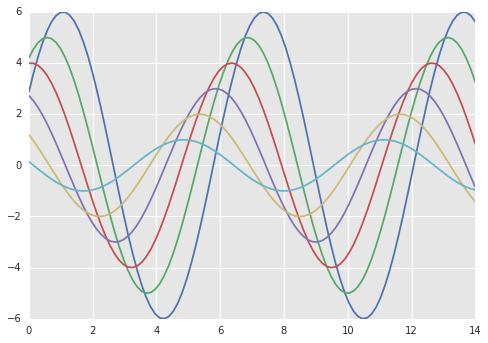
\includegraphics[width=0.7\linewidth]{images/aesthetics_31_0}
\end{figure}

\end{frame}
\section{Scaling plot elements with plotting\_context() and set\_context()}
%====================================%
\begin{frame}[fragile]
	\frametitle{Seaborn Workshop}
	\large
	\begin{itemize}
\item Scaling plot elements with \texttt{plotting\_context()} and \texttt{set\_context()}
\item A separate set of parameters control the scale of plot elements, which should let you use the same code to make plots that are suited for use in settings where larger or smaller plots are appropriate.
	\end{itemize}

\end{frame}
%====================================%
\begin{frame}[fragile]
	\frametitle{Seaborn Workshop}
	\large
First let’s reset the default parameters by calling \texttt{set()}:
\begin{verbatim}
sns.set()
\end{verbatim}
\begin{itemize}
\item The four preset contexts, in order of relative size, are paper, notebook, talk, and poster.
\item The notebook style is the default, and was used in the plots above.
\end{itemize}

\end{frame}
%====================================%
\begin{frame}[fragile]
	\frametitle{Seaborn Workshop}
	\large
\begin{verbatim}
sns.set_context("paper")
plt.figure(figsize=(8, 6))
sinplot()
\end{verbatim}

\begin{figure}
	\centering
	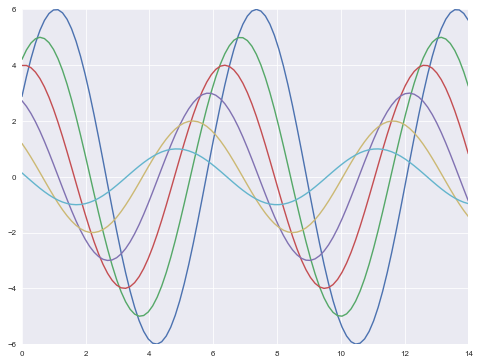
\includegraphics[width=0.7\linewidth]{images/aesthetics_35_0}
\end{figure}


\end{frame}
%====================================%
\begin{frame}[fragile]
	\frametitle{Seaborn Workshop}
	\large
\begin{verbatim}
	sns.set_context("talk")
	plt.figure(figsize=(8, 6))
	sinplot()
\end{verbatim}

\begin{figure}
	\centering
	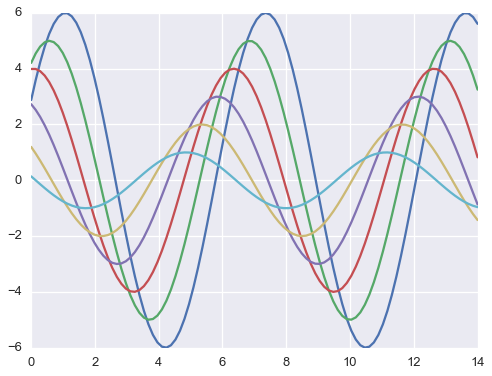
\includegraphics[width=0.7\linewidth]{images/aesthetics_36_0}
\end{figure}
\end{frame}
%====================================%
\begin{frame}[fragile]
	\frametitle{Seaborn Workshop}
	\large
\begin{verbatim}
sns.set_context("poster")
plt.figure(figsize=(8, 6))
sinplot()
\end{verbatim}

\begin{figure}
	\centering
	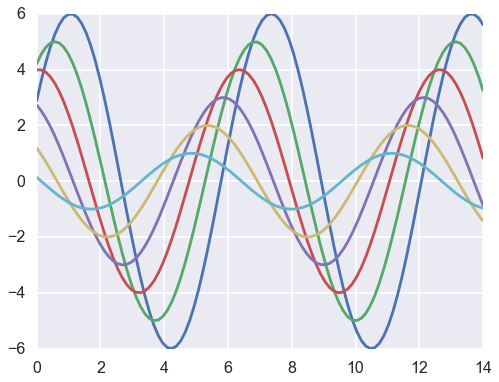
\includegraphics[width=0.7\linewidth]{images/aesthetics_37_0}
\end{figure}

\end{frame}
%====================================%
\begin{frame}[fragile]
	\frametitle{Seaborn Workshop}
	\large 
\begin{itemize}
\item Most of what you now know about the style functions should transfer to the context functions.
\item You can call \texttt{set\_context()} with one of these names to set the parameters, and you can override the parameters by providing a dictionary of parameter values.
\end{itemize}
\end{frame}
%====================================%
\begin{frame}[fragile]
	\frametitle{Seaborn Workshop}
	\large
	\begin{itemize}
\item You can also independently scale the size of the font elements when changing the context. 
\item This option is also available through the top-level \texttt{set()} function.
	\end{itemize}

\end{frame}
%====================================%
\begin{frame}[fragile]
	\frametitle{Seaborn Workshop}
	\large
\begin{verbatim}
sns.set_context("notebook", font_scale=1.5, rc={"lines.linewidth": 2.5})
sinplot()
\end{verbatim}

\begin{figure}
	\centering
	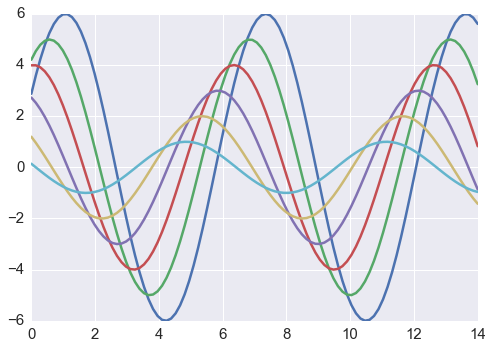
\includegraphics[width=0.7\linewidth]{images/aesthetics_39_0}
\end{figure}

Similarly (although it might be less useful), you can temporarily control the scale of figures nested under a with statement.
\end{frame}
%====================================%
\end{document}